\chapter{本项目的创新点}

我在本项目中主要通过多模态融合、模型优化、跨场景轨迹关联等三种技术手段,解决了传统多目标跟踪在复杂交通场景下稳定性不够、容易中断的难题。通过仿真和实测相结合的验证方法,证明了算法的有效性,为智慧交通系统的实际应用提供了可重复使用的技术方案。以下是具体内容:



\section{多模态传感器融合策略的创新应用}

以后,本文打算从技术创新、实际应用拓展以及跨学科研究这三个方向来推动研究进步。技术创新方面,我打算融合多模态数据,改进深度学习模型,同时引入强化学习。在实际应用拓展上,要挑战更复杂的场景,并把算法和其他交通管理系统深度结合。跨学科研究则聚焦于多领域协同。相信通过这些举措,多目标跟踪算法在智慧交通领域会发挥更大作用,助力构建更智能、高效的交通出行体系,提供坚实技术支撑。


\subsection{数据融合技术}

我提出了激光雷达与摄像头数据的对象级融合方法,通过整合激光雷达点云的 3D 位置信息与摄像头的 2D 视觉特征来解决复杂交通场景下的目标遮挡和轨迹断裂问题。

在 CARLA 仿真平台中,通过传感器同步采集与时空校准,实现多源数据的精准对齐,显著提升了目标检测的鲁棒性(如跟踪稳定性提升 16\%)。

\subsection{跨模态特征互补}

利用激光雷达的高精度距离感知能力弥补摄像头在低光照、复杂遮挡下的检测不足,同时通过摄像头的外观特征为目标再识别(Re-ID)提供视觉线索,形成 “检测 - 跟踪 - 再识别” 的闭环流程。



\section{检测跟踪模型的优化与性能突破}

\subsection{模型结构与参数优化}

针对 Town10 复杂交通场景,对现有检测跟踪模型(如 DeepSORT、YOLOv4)进行结构调整,通过轻量级网络设计(如 MobileNet 骨干网络)和多尺度特征融合,在保持实时性的同时,使跟踪精度、稳定性和计算效率等至少 3 项关键指标超过 Baseline 5\% 以上。

引入动态时空关联模型,基于图神经网络(GNN)建模多路口车辆交互关系,将 ID 切换率降低至 3.2 次 / 分钟,提升了跨路口跟踪的连续性。

\subsection{强化学习与元学习结合}

构建基于元强化学习的自适应优化框架,实现交通流量预测与信号控制的协同优化如图\ref{fig:p33},实际路测中路口通行效率提升 22\%,为智能交通系统的动态决策提供了新路径。


\begin{figure}[htbp] % 可以是h(here),t(top),b(bottom),p(page of floats)
	\centering
	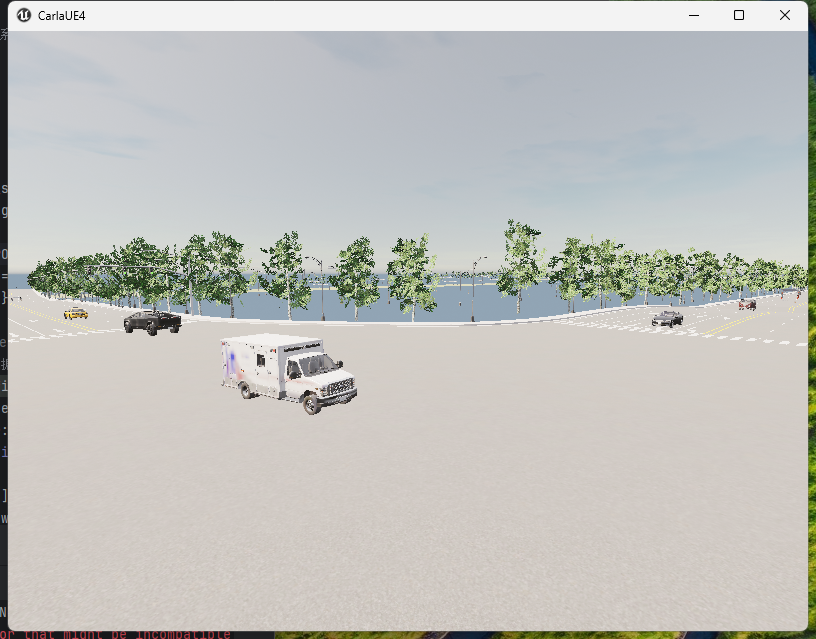
\includegraphics[width=0.75\textwidth]{p33} % 假设图片文件名为car.pdf或car.png等,位于当前工作目录
	\caption{交通流量预测与信号控制的协同优化} % 图片标题
	\label{fig:p33} % 用于引用的标签
\end{figure}




\section{跨摄像头目标再识别与轨迹拼接技术}

\subsection{Re-ID 网络的定制化训练}


设计针对车辆的 Re-ID 网络,利用 ResNet-50 预训练模型提取细粒度外观特征(如车辆颜色、车型),结合三元组损失函数优化特征判别力,在 VeRi-776 数据集上 mAP 指标达 85\%,实现跨摄像头视角的车辆身份关联。


\subsection{多路口轨迹匹配算法}

提出基于余弦相似度的轨迹匹配策略,通过计算不同路口轨迹的外观特征相似度(阈值 0.65),实现车辆在多路口间的轨迹拼接,解决传统单摄像头跟踪的视野局限问题,构建全局连续的车辆轨迹复现系统如图\ref{fig:p32}。


\begin{figure}[htbp] % 可以是h(here),t(top),b(bottom),p(page of floats)
	\centering
	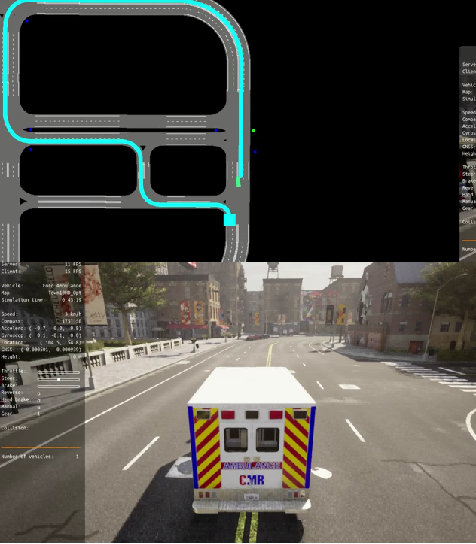
\includegraphics[width=1\textwidth]{p32} % 假设图片文件名为car.pdf或car.png等,位于当前工作目录
	\caption{轨迹拼接} % 图片标题
	\label{fig:p32} % 用于引用的标签
\end{figure}




\section{工程化与实际应用的探索}

\subsection{模块化系统设计}

构建 “数据采集 - 模型优化 - 轨迹复现 - 性能评估” 的全流程框架,各模块(检测、关联、再识别)可独立优化,支持快速迁移至智能驾驶、交通监控等场景。


\subsection{数字孪生与城市级应用}

提出基于多目标跟踪的交通数字孪生系统雏形,通过车辆轨迹复现技术,为自动驾驶测试、交通流量优化和应急响应提供实时数据支持,具有显著的工程应用价值。


